\documentclass[12 pt]{report}
\usepackage{tikz,amsmath,pgfplots}
\usetikzlibrary{tikzmark,calc}
\pgfplotsset{compat=1.17}

\begin{document}
    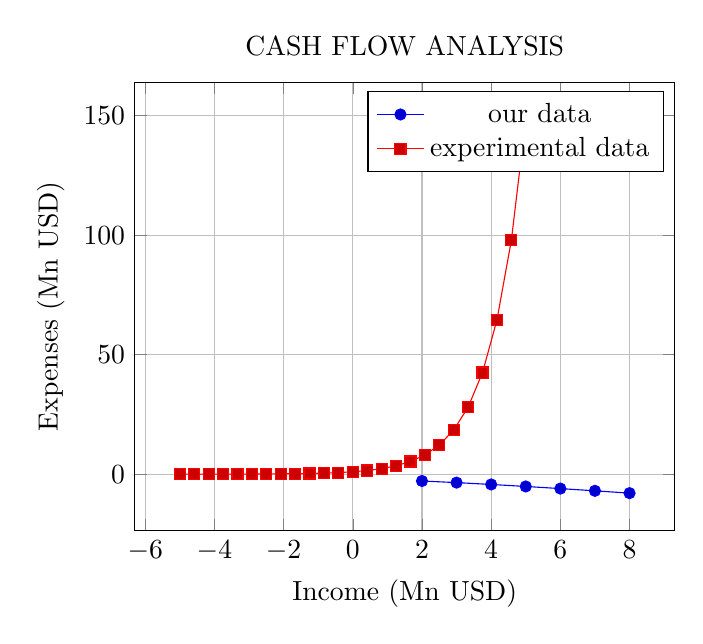
\begin{tikzpicture}
           \begin{axis}[
                    xlabel=Income (Mn USD), 
                    ylabel=Expenses (Mn USD), 
                    grid,
                    title=CASH FLOW ANALYSIS]
               \addplot coordinates {
		            (2,-2.8559703)
		            (3,-3.5301677)
		            (4,-4.3050655)
	            	(5,-5.1413136)
		            (6,-6.0322865)
		            (7,-6.9675052)
		            (8,-7.9377747)
	            };
	            \addlegendentry{our data}
	            \addplot {e^x};
	            \addlegendentry{experimental data}
           \end{axis}
    \end{tikzpicture}
    
    
    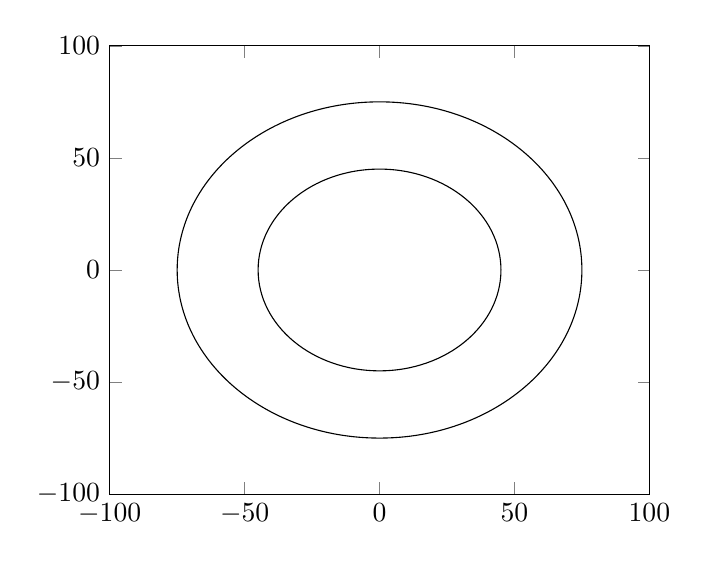
\begin{tikzpicture}
       \begin{axis}[xmin=-100, xmax=100,ymin=-100, ymax=100]
        \draw (axis cs:0,0) circle[radius=75];
        \draw (axis cs:0,0) circle[radius=45];
    \end{axis}  
    \end{tikzpicture}
    \newpage
   \tikzset{every node/.style={outer sep=2pt}}
    \[
    \tikzmarknode{De}{\text{De}} = \tikzmarknode{Re}{\text{Re}}\sqrt{\frac{{\tikzmarknode{D}{D}}}{\tikzmarknode{2RC}{2R_C}}}
    \]
    
    \begin{tikzpicture}[remember picture,overlay]
        \draw[->] (De.north) to[out=90,in=60,looseness=1.5] ($(De)+(-1,0)$) node[left] {Dean number};
        \draw[->] (Re.north) to[out=90,in=180] ($(Re)+(1.2,1.2)$) node[right] {Reynolds number};
        \draw[->] (D.east) to[out=45,in=190] ($(D)+(1.5,-1)$) node[right] {Hydraulic diameter};
        \draw[->] (2RC.south) to[out=-90,in=0] ($(2RC)+(-1.5,-1)$) node[left] {Path curvature radius};
    \end{tikzpicture} 
    \vspace{30 mm}
    
    \[
    \tikzmarknode{Re}{\text{Re}}=\frac{{\tikzmarknode{IF}{\text{Interial force}}}}{{\tikzmarknode{VF}{\text{Viscous force}}}}=\frac{{   \tikzmarknode{m}{\text{m}} \tikzmarknode{a}{\text{a}}     }} {  \tikzmarknode{Tau}{\tau} \tikzmarknode{A}{\text{A}}  } = \frac{{   \tikzmarknode{m_dot}{\dot{\text{m}}} \tikzmarknode{u}{\text{u}}     }} {  \tikzmarknode{Tau}{\tau} \tikzmarknode{A}{\text{A}}  } = \frac{\rho \ A\ u^2}{\mu \big( \frac{u}{L}\big)A}=\frac{\rho \ u\ L}{\mu}=\frac{u\ L}{\nu}
    \]
    
    \begin{tikzpicture}[remember picture,overlay]
        \draw[->] (m_dot.north) to[out=90,in=180, looseness=1] ($(m_dot)+(0.65,1.5)$) node [right] {$\rho$Q  $= \rho \text{Au}$};
        \draw[->] (a.north) to[out=70, in=160, looseness=1] ($(a)+(0.4,0.8)$) node[right] {$\frac{u}{t}$};
        \draw[->] (Tau.south) to[out=-110, in=0, looseness=1] ($(Tau)+(-1,-1)$) node [left] {$ \mu \ \frac{u}{L} \Leftarrow \mu \ \frac{du}{dy}$};
    \end{tikzpicture} 
    \newpage

    \[
    \tikzmarknode{F}{\text{Fr}}=\sqrt{\frac{{\tikzmarknode{IF}{\text{Interial force}}}}{{\tikzmarknode{GF}{\text{Gravity force}}}}}=\sqrt{\frac{\rho \ A\ u^2}{\tikzmarknode{m}{m}\ g}}=\sqrt{\frac{\rho \ A\ u^2}{\rho\ A\ L\ g}}=\frac{u}{\sqrt{Lg}}
    \]
    \begin{tikzpicture}[remember picture,overlay]
        \draw[->] (m.south) to[out=-90, in=90, looseness=1.5] ($(m)+(-1,-1)$) node[below] {$\rho \ V\ \simeq \rho\ L^3 \simeq \rho \ AL$};
    \end{tikzpicture} 
    \newpage
     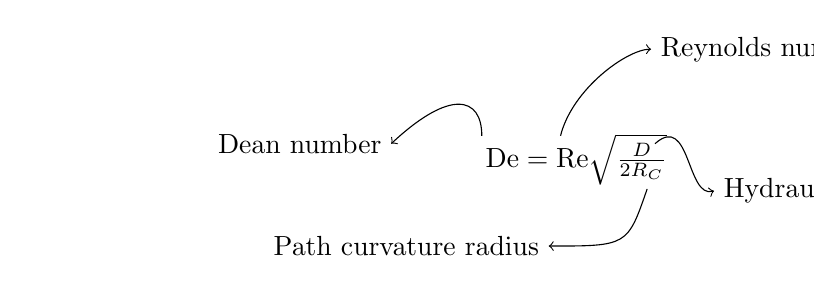
\begin{tikzpicture}[]
            $\mathrm{De}= \mathrm{Re}\sqrt{\frac{D}{2R_C}}$
            \draw[->] (-1.35,0.4) ..controls (-1.2,1) and (-0.5,1.5) .. (-0.2,1.5) node[right] {Reynolds number};
            \draw[->] (-2.35,0.4) .. controls (-2.35,0.9) and (-2.75,1)   .. (-3.5,0.3) node[left] {Dean number};
            \draw[->] (-0.15,0.3) .. controls (0.3,0.7) and (0.25,-0.4) .. (0.6,-0.3) node[right] {Hydraulic diameter};
            \draw[->] (-0.25,-0.275) .. controls (-0.5,-1)  .. (-1.5,-1) node[left] {Path curvature radius};
    \end{tikzpicture}
    

\tikzset{every picture/.style={line width=0.75pt}} %set default line width to 0.75pt        

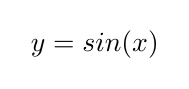
\begin{tikzpicture}[x=0.75pt,y=0.75pt,yscale=-1,xscale=1]
%uncomment if require: \path (0,310); %set diagram left start at 0, and has height of 310

% Plotting does not support converting to Tikz

% Text Node
\draw (419,54.4) node [anchor=north west][inner sep=0.75pt]    {$y=sin( x)$};


\end{tikzpicture}

   
\end{document} 